% $Id: INF_Poster_example.tex 7714 2011-08-31 17:34:46Z tkren $
%
% TU Wien - Faculty of Informatics
% poster template
%
% This template is using the beamer document class and beamerposter package, see
% <http://www.ctan.org/tex-archive/macros/latex/contrib/beamer/>
% <http://www.ctan.org/tex-archive/macros/latex/contrib/beamerposter/>
% <http://www-i6.informatik.rwth-aachen.de/~dreuw/latexbeamerposter.php>
%
% For questions and comments send an email to
% Thomas Krennwallner <tkren@kr.tuwien.ac.at>
%

\documentclass[final,hyperref={pdfpagelabels=true}]{beamer}

\usepackage{minted}
\usepackage{TUINFPST}
\usepackage{listings}
\usepackage{wrapfig}

%\title[Computational Intelligence]{Interactive Computer Generated Architecture}
% if you have a long title looking squeezed on the poster, just force
% some distance:
\title[Software Engineering \& Internet Computing]{%
  A Weather Ontology for \\[0.2\baselineskip]%
  Predictive Control in Smart Homes %\\[0.2\baselineskip]%
}
\author[paulchen@rueckgr.at]{Paul Staroch}
\institute[]{%
  Technische Universit{\"a}t Wien\\[0.25\baselineskip]
  Institut für computergestützte Automation\\[0.25\baselineskip]
  Arbeitsbereich: Automation Systems Group\\[0.25\baselineskip]
  BetreuerIn: Ao.Univ.-Prof. Dipl.-Ing. Dr.techn. Wolfgang Kastner\\[0.25\baselineskip]
  AssistentIn: Dipl.-Ing. Mario Kofler
}
\titlegraphic{
\includegraphics[height=52mm]{figures/183-1.pdf}}
\date[\today]{\today}
\subject{epilog}
\keywords{my kwd1, my kwd2} % TODO

%%%%%%%%%%%%%%%%%%%%%%%%%%%%%%%%%%%%%%%%%%%%%%%%%%%%%%%%%%%%%%%%%%%%%%%%%%%%%%%%%%%%%%

% Display a grid to help align images 
%\beamertemplategridbackground[12.7mm] % TODO remove

% play around with the background colors
% \setbeamercolor{background canvas}{bg=yellow}

% use a background picture
%\usebackgroundtemplate{%
%  
\includegraphics[width=\paperwidth]{logo_KBS_2_CMYK}
%}

% play around with block colors
\setbeamercolor{block body}{fg=black,bg=white}
\setbeamercolor{block title}{fg=TuWienBlue,bg=white}

\definecolor{TuWienBlueLight}{cmyk}{.1,.1,.1,.3}
\definecolor{listingBottom}{cmyk}{.1,.1,.1,.1}

\setbeamertemplate{block begin}{
  \begin{beamercolorbox}{block title}%
    
\begin{tikzpicture}%
      \node[draw,rectangle,line width=3pt,rounded corners=0pt,inner sep=0pt,shade,top color=white,bottom color=TuWienBlueLight]{%
        \begin{minipage}[c][2cm]{\linewidth}
          \centering\textbf{\insertblocktitle}
        \end{minipage}
      };
    \end{tikzpicture}%
  \end{beamercolorbox}
  \vspace*{1cm}
  \begin{beamercolorbox}{block body}%
}

\setbeamertemplate{block end}{
  \end{beamercolorbox}
  \vspace{2cm}
}

% setup postit
\setbeamercolor{postit}{fg=black,bg=yellow} 
\newenvironment{postit}
{\begin{beamercolorbox}[sep=1em,wd=7cm]{postit}}
{\end{beamercolorbox}}


% for crop marks, uncomment the following line
%\usepackage[cross,width=88truecm,height=123truecm,center]{crop} % TODO

%%%%%%%%%%%%%%%%%%%%%%%%%%%%%%%%%%%%%%%%%%%%%%%%%%%%%%%%%%%%%%%%%%%%%%%%%%%%%%%%%%%%%%

%\lstset{frame=trbl,basicstyle=\scriptsize,moredelim=**[is][{\btHL[fill=green!20]}]{@@}{@@},}
%\lstset{frame=trBL,basicstyle=\normalsize}

% \setlength{\parskip}{15em}

\begin{document}

% We have a single poster frame.
\begin{frame}[fragile]
  \begin{columns}[t]
    % ---------------------------------------------------------%
    % Set up a column
    \begin{column}{.45\textwidth}
      \begin{block}{Smart homes and ontologies}
	\emph{Smart homes} are dwellings that are equipped with
	some kind of intelligence that enables them to perform tasks
	on its own without human intervention. Some of their goals are:

	\begin{itemize}
	  \item Supporting the inhabitants in their routine tasks.
	  \item Maintaining or increase the inhabitant's comfort.
          \item Reducing the overall energy consumption.
        \end{itemize}

	Many smart home systems suffer from several shortcomings:
	\begin{itemize}
	  \item Smart home systems tend to be very complex.
	  \item Optimisations and customisations imply a huge effort.
	  \item Smart homes are less powerful or flexible than desired.
	\end{itemize}

	One approach to overcome these problems is to utilise a knowledge
	base built using \emph{OWL}, like in \emph{ThinkHome}~\cite{CR2011-TH_Journal}.
      \end{block}

      \begin{block}{Why introduce a weather data model?}
        \begin{wrapfigure}{r}{.45\textwidth}
	  \centering
	  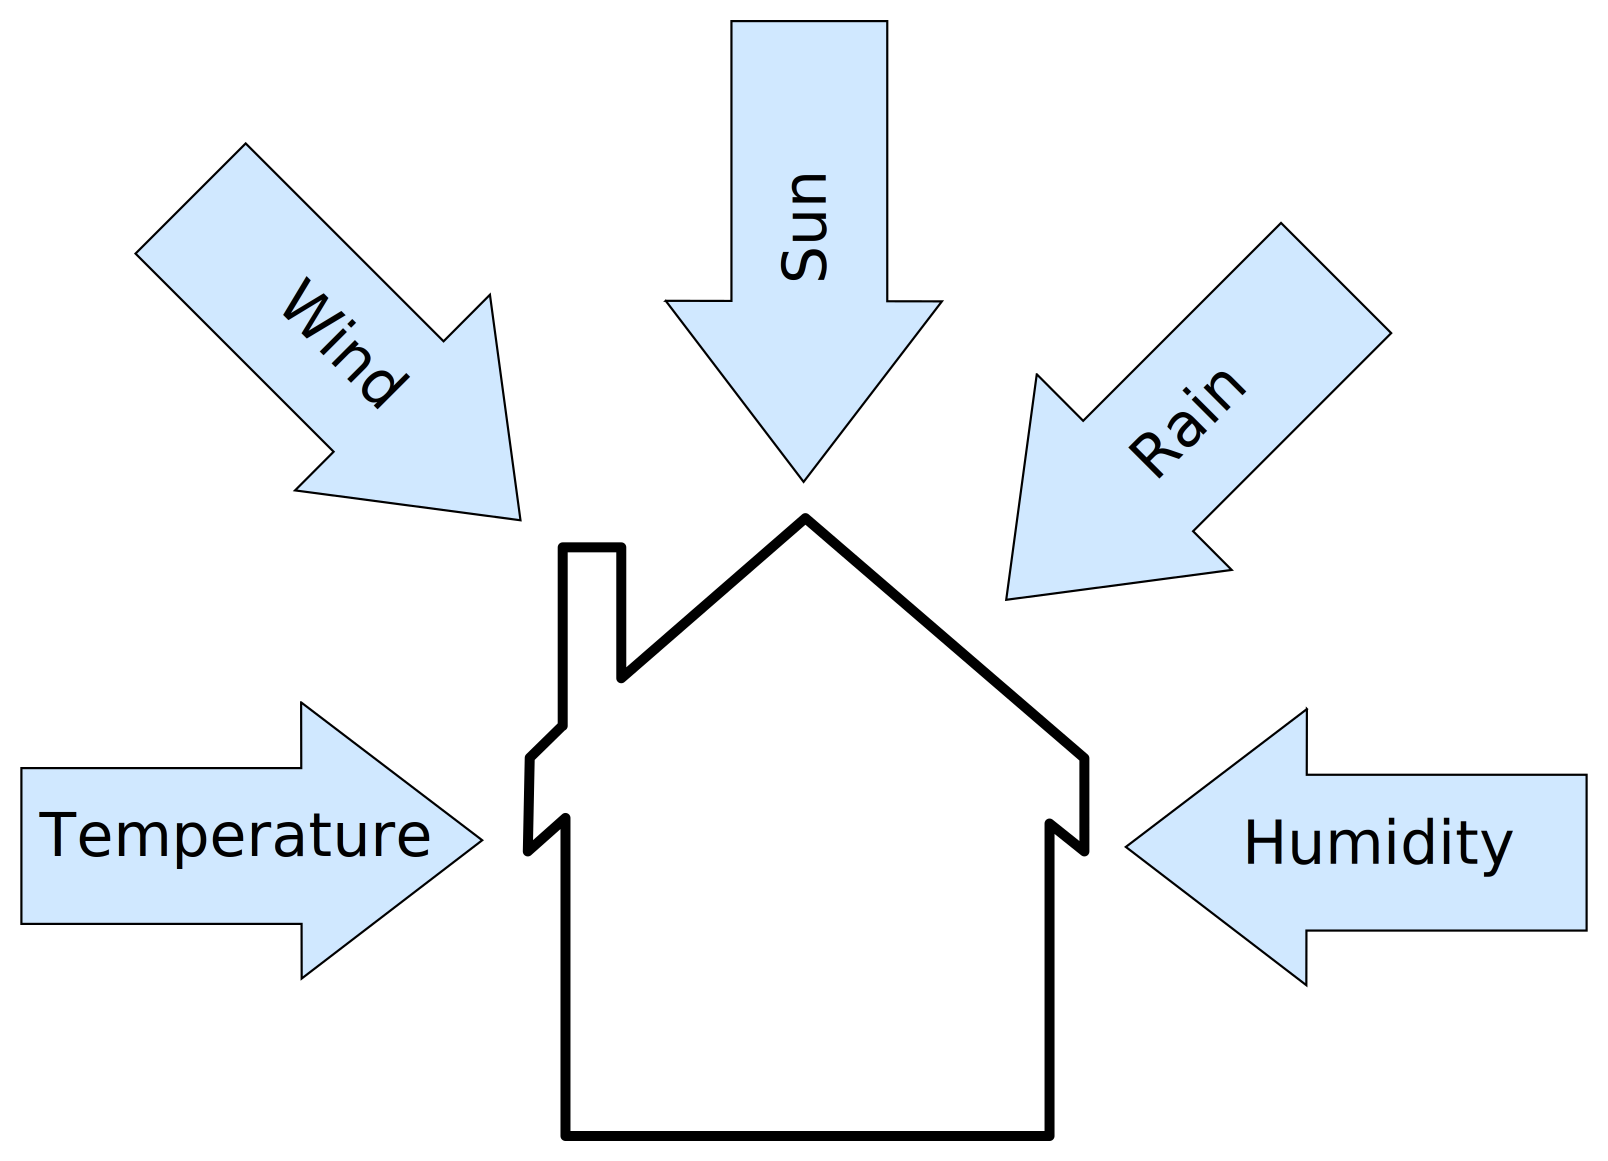
\includegraphics[width=.45\textwidth]{figures/inkscape/house}
	\end{wrapfigure}

	\mbox{Weather has a wide influence on}
	\mbox{a dwelling. Introducing \emph{SmartHome-}}
	\mbox{\emph{Weather}, a data model for current}
	\mbox{for current and future weather}
	\mbox{states, enables a smart home to}
	\mbox{utilise various aspects of this}
	\mbox{influence to make a set of control}
	decisions, regarding e.g.
	\begin{itemize}
  	  \item heating, ventilation, and air conditioning (\emph{HVAC}),
	  \item the utilisation of solar and wind power,
	  \item irrigation, or
	  \item preparations for severe weather, e.g. by closing windows or retracting awnings.
	\end{itemize}

	Data about weather states is gathered from local sensors and Internet weather services.
      \end{block}

      \begin{block}{Preliminary work}
	The work preceding the development of \emph{SmartHomeWeather} followed this methodological approach:
	\begin{itemize}
	  \item Existing weather ontologies were evaluated; none of them were found to be suitable to be used in smart homes.
	  \item Particular ways were identified in which weather data can be used in smart homes. This led to the set of weather elements supported by the ontology (temperature, humidity…).
	  \item Among approaches for building ontologies from scratch, \emph{METHONTOLOGY}~\cite{Methontology} was selected to be applied to the development process of \emph{SmartHomeWeather}.
	  \item A selection of Internet weather services was evaluated. The \emph{API} provided by the \emph{Norwegian Meteorological Institute} is used as an example.
	\end{itemize}
      \end{block}

      \begin{block}{The \emph{SmartHomeWeather} ontology}
	The \emph{SmartHomeWeather} ontology is built around five top-level
	concepts which together with their sub-concepts form a model for
	maintaining data about current and future weather and perform efficient
	\emph{OWL} reasoning on it:
	
	\begin{itemize}
	  \item A \emph{Weather phenomenon} describes a certain weather
		  element (e.g.\ temperature or humidity).
	\end{itemize}
      \end{block}
    \end{column}
    % ---------------------------------------------------------%
    % end the column

    % ---------------------------------------------------------%
    % Set up a column 
    \begin{column}{.45\textwidth}
      \begin{block}{The \emph{SmartHomeWeather} ontology (cont.)}
	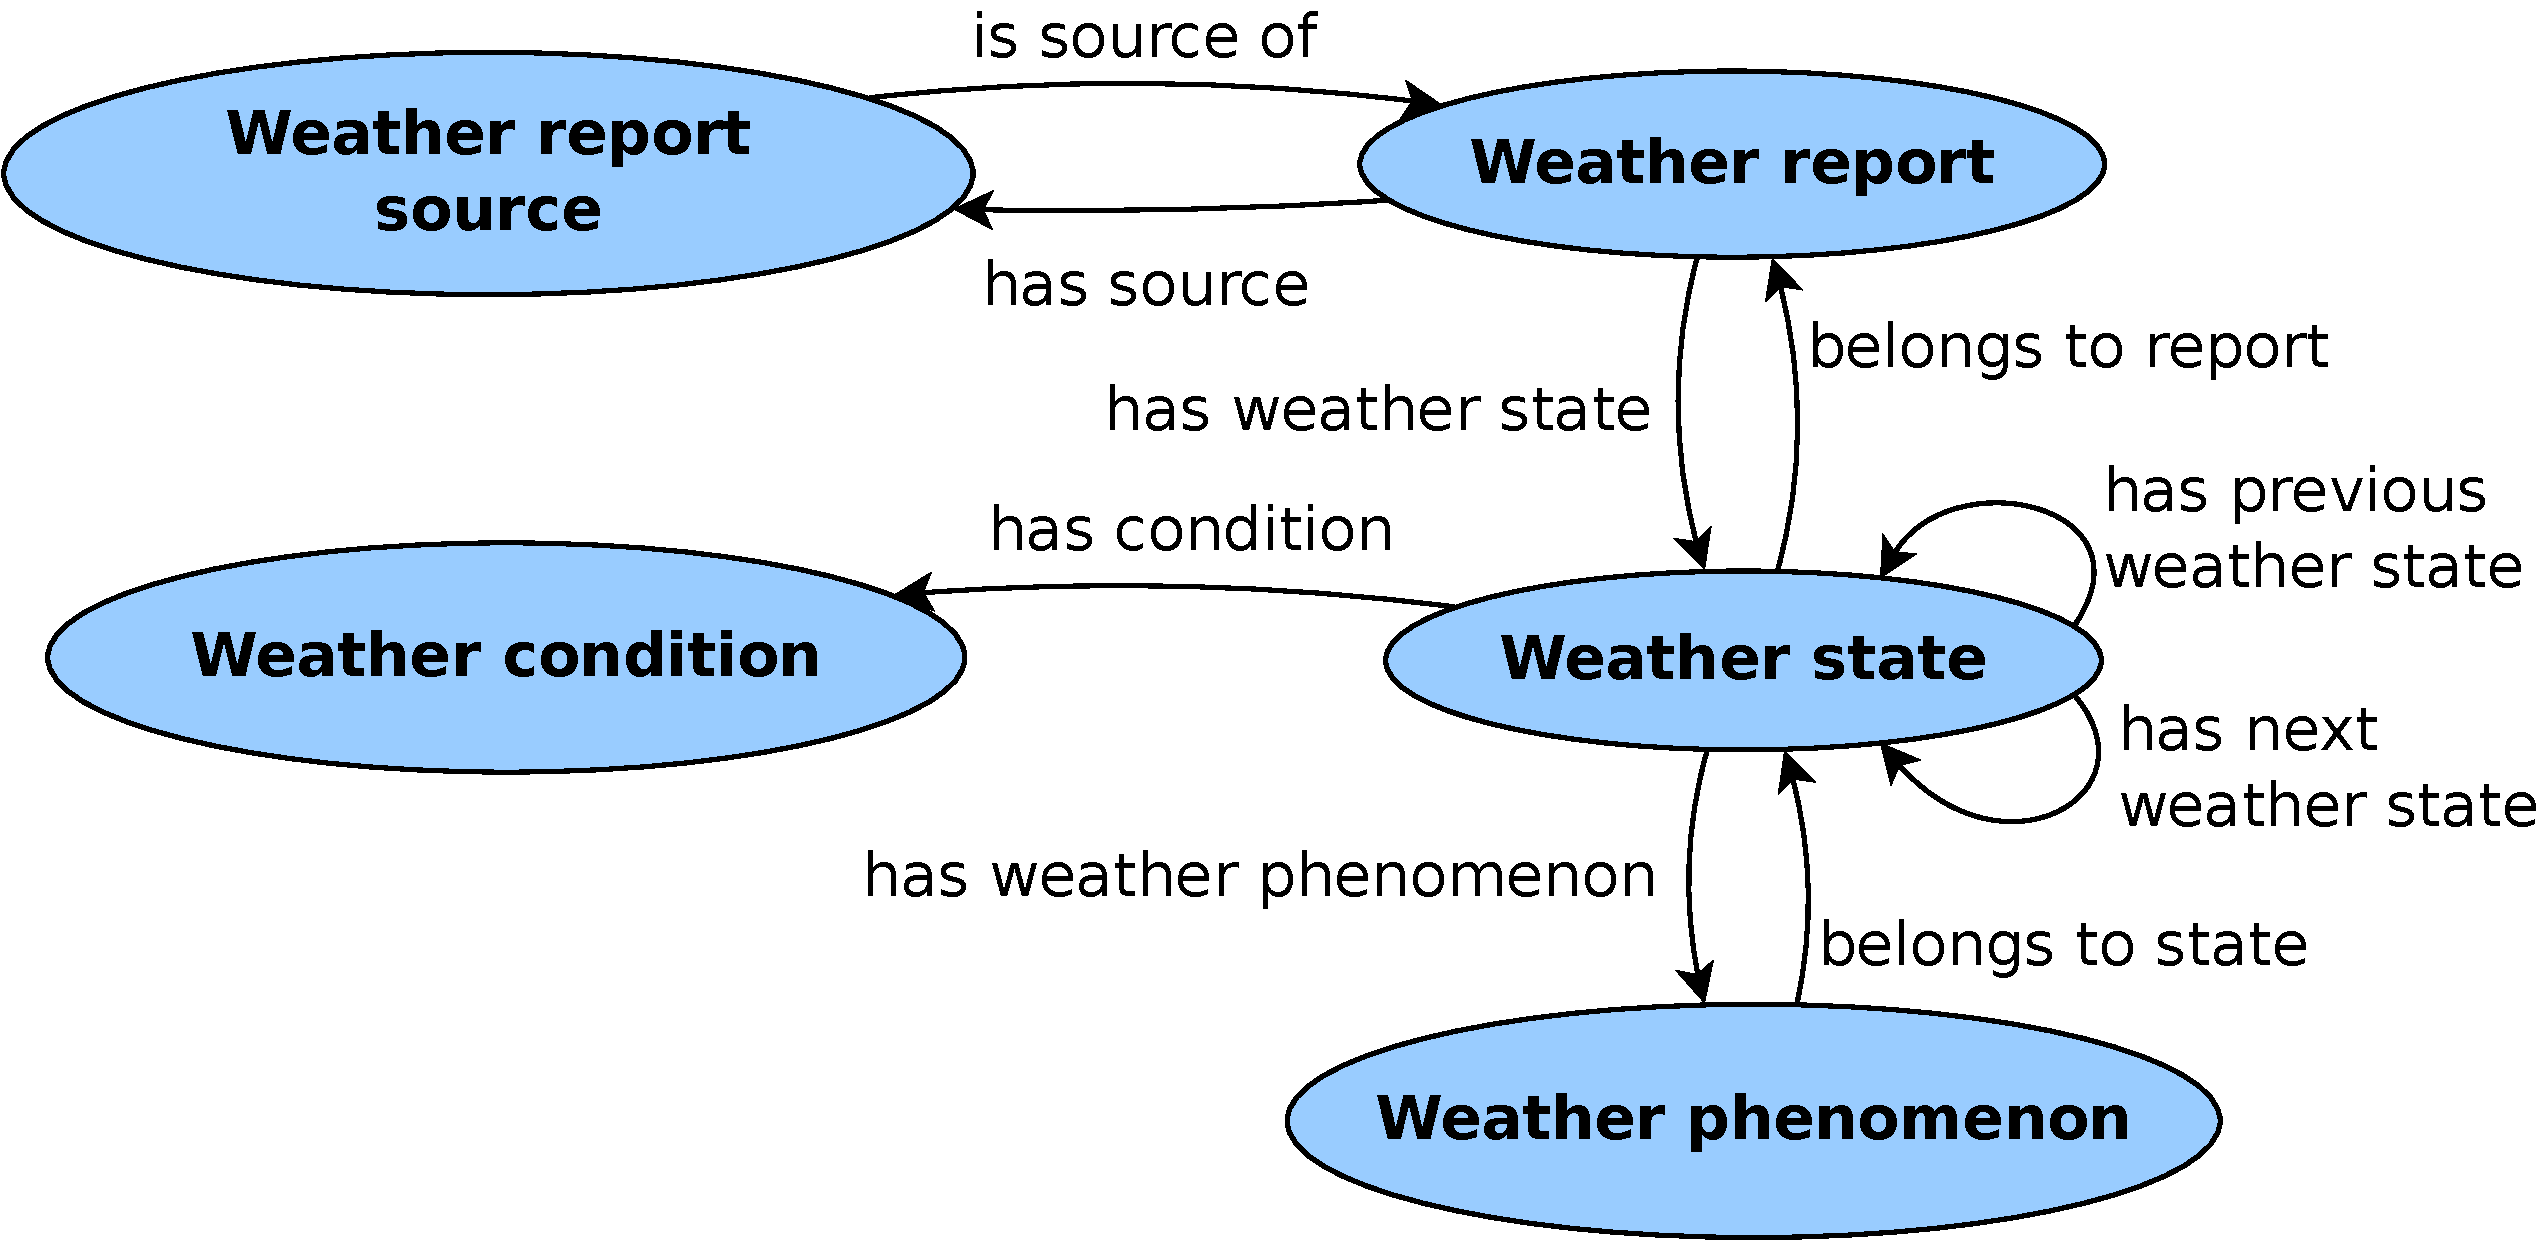
\includegraphics[width=\textwidth]{figures/dia/binary-relations}
	\begin{itemize}
	  \item \emph{Weather condition} is a one-word description of the
		  weather situation (e.g.\ ``Sun'' or ``Fog'').
	  \item A \emph{Weather state} describes the weather situation as a
		  set of instances of \emph{Weather phenomenon}.
          \item A \emph{Weather report} describes the weather for a certain
		  point of time.
	  \item A \emph{Weather report source} (sensor or Internet service)
		  provides weather data.
	\end{itemize}

	There are several sub-concepts which are inferred using \emph{OWL} reasoning, e.g.\ 
	\begin{itemize}
	  \item \emph{Temperature} of \emph{Weather phenomenon} (which again has sub-concepts, e.g.\
		  \emph{Room temperature}),
	  \item \emph{Pleasant temperature weather} of \emph{Weather state}, and
	  \item \emph{Short range weather report} of \emph{Weather report}.
	\end{itemize}

	The data model can be queried using \emph{SPARQL} queries, e.g.\ to query all \emph{Weather report}s describing room temperature:

	\vspace{10mm}
	\begin{tikzpicture}%
          \node[draw,rectangle,line width=3pt,rounded corners=0pt,inner sep=0pt,shade,top color=white,bottom color=listingBottom]{%
	    \begin{minipage}{\textwidth}
	      \hspace{5mm}
              \begin{minipage}{\textwidth}
              \vspace{5mm}
    	      \begin{minted}{sparql}
SELECT ?r
WHERE {
    ?r weather:hasWeatherState ?s.
    ?s weather:hasWeatherPhenomenon ?t.
    ?t a weather:RoomTemperature.
}
    	      \end{minted}
    	      \vspace{5mm}
	      \end{minipage}
            \end{minipage}
	  };
	\end{tikzpicture}
	\vspace{-12mm}
	
	The \emph{Weather Importer}, a Java application, imports weather data from sensors and services
	into the ontology.
      \end{block}
      
      \begin{block}{Future work}
	Interoperation with other data sources, e.g.:
	\begin{itemize}
	  \item Minimising costs for electrical power based on weather data and varying costs for electrical power over time.
	  \item Improving decision making based on both weather data and the buildings' inhabitants' actions.
	  \item Learning from weather situations and their influence on the dwelling.
	\end{itemize}
      \end{block}

      \begin{block}{References}
        \footnotesize
	\bibliographystyle{thesis}
	\bibliography{references}
      \end{block}
    \end{column}
    % ---------------------------------------------------------%
    % end the column
  \end{columns}

%  \begin{tikzpicture}[remember picture,overlay]
%    \node[inner sep=0pt,xshift=-30cm,yshift=23cm] at (current page.east) {%
%      \begin{postit}%
%        Post-It time!%
%      \end{postit}%
%    }; 
%  \end{tikzpicture}
  
\end{frame}

\end{document}


%%% Local Variables:
%%% TeX-PDF-mode: t
%%% TeX-debug-bad-boxes: t
%%% TeX-master: t
%%% TeX-parse-self: t
%%% TeX-auto-save: t
%%% reftex-plug-into-AUCTeX: t
%%% End:
